
\documentclass[journal,transmag]{IEEEtran}
\hyphenation{op-tical net-works semi-conduc-tor}

\usepackage{enumitem}

% *** GRAPHICS RELATED PACKAGES ***
%
\ifCLASSINFOpdf
   \usepackage[pdftex]{graphicx}
  % declare the path(s) where your graphic files are
  % \graphicspath{{../pdf/}{../jpeg/}}
  % and their extensions so you won't have to specify these with
  % every instance of \includegraphics
  % \DeclareGraphicsExtensions{.pdf,.jpeg,.png}
\else
  % or other class option (dvipsone, dvipdf, if not using dvips). graphicx
  % will default to the driver specified in the system graphics.cfg if no
  % driver is specified.
  % \usepackage[dvips]{graphicx}
  % declare the path(s) where your graphic files are
  % \graphicspath{{../eps/}}
  % and their extensions so you won't have to specify these with
  % every instance of \includegraphics
  % \DeclareGraphicsExtensions{.eps}
\fi
% graphicx was written by David Carlisle and Sebastian Rahtz. It is
% required if you want graphics, photos, etc. graphicx.sty is already
% installed on most LaTeX systems. The latest version and documentation
% can be obtained at: 
% http://www.ctan.org/pkg/graphicx
% Another good source of documentation is "Using Imported Graphics in
% LaTeX2e" by Keith Reckdahl which can be found at:
% http://www.ctan.org/pkg/epslatex
%
% latex, and pdflatex in dvi mode, support graphics in encapsulated
% postscript (.eps) format. pdflatex in pdf mode supports graphics
% in .pdf, .jpeg, .png and .mps (metapost) formats. Users should ensure
% that all non-photo figures use a vector format (.eps, .pdf, .mps) and
% not a bitmapped formats (.jpeg, .png). The IEEE frowns on bitmapped formats
% which can result in "jaggedy"/blurry rendering of lines and letters as
% well as large increases in file sizes.
%
% You can find documentation about the pdfTeX application at:
% http://www.tug.org/applications/pdftex





\begin{document}

\title{\textsc{Resistencia de materiales a tensión }}

\author{
\IEEEauthorblockN{Tensile Strength of Materials  }
\IEEEauthorblockA{Pontificia Universidad Javeriana, Bogotá, Colombia}
\IEEEauthorblockA{Naryi Vanesa Medina Castelo , Claudio Rodrigo Carranza Navarro, William A. Gómez}
\IEEEauthorblockA{Daniel Alejandro Jiménez Giraldo, Nicolle Agudelo Padilla}

}
% The paper headers
\markboth{BIOMECÁNICA. Noviembre 03~2022}%
{Shell \MakeLowercase{\textit{et al.}}: Bare Demo of IEEEtran.cls for IEEE Transactions on Magnetics Journals}
\IEEEtitleabstractindextext{%

	\begin{abstract}
El estudio de la mecánica de materiales nos brinda las herramientas necesarias para analizar y diseñar diversos materiales y/o estructuras con el objetivo de caracterizar sus esfuerzos y deformaciones. Así pues, con este fin, en la presente práctica experimental se realizó una prueba de tracción simple a un grupo de cinco probetas hechas en ácido poliláctico (PLLA) a través de impresión 3D, a las cuales se las varió la densidad de relleno entre el 40\% y el 100\%; Posteriormente, los datos fueron analizados y graficados, con el propósito de identificar el módulo de Young, el esfuerzo de fluencia y el esfuerzo máximo del material; Todo lo anterior, regido bajo la normativa ISO 527 para ensayos de tracción para plásticos. 

	\end{abstract}
	\begin{IEEEkeywords}
	Tracción, Módulo de Young, Esfuerzo, PLLA, Deformación,  ISO 527 .
	 	\end{IEEEkeywords}}


\maketitle
\IEEEdisplaynontitleabstractindextext
\IEEEpeerreviewmaketitle


\section{Introducción}


Dentro de la bioingeniería y en general las diversas áreas del conociendo enfocadas en el desarrollo de cualquier dispositivo, maquina, estructura, etc. es indispensable conocer las características mecánicas de aquellos materiales que componen dicho equipo, con el fin de asegurar que este sea seguro y eficaz, pero sobre todo adecuado para lo que se plantea usar, es decir que, una vez este se cargue, no se deforme excesivamente frente a las condiciones establecidas por el entorno operativo en el que se encuentra y que por consiguiente, no se quiebre.  

Así pues, el estudio de la resistencia de materiales permite seleccionar el material adecuado con el fin de que la estructura sea segura frente a los efectos combinados de las fuerzas y momentos, sin embargo, para elegir el material adecuado es necesario conocer las propiedades mecánicas de este material en diferentes condiciones de carga. Si un cuerpo se encuentra sometido a fuerzas externas, este sufrirá una deformación, es decir, un cambio de forma local, esta deformación dependerá de las distintas configuraciones de carga que le sean aplicadas, es decir, de la magnitud, la dirección y la duración de las fuerzas externas aplicadas, la ideal que de las propiedades del material del cuerpo y de condiciones ambientales. [1] 

Con el fin de determinar las propiedades mecánicas de los materiales se realizan diversas pruebas mecánicas, en las cuales se aplican distintos tipos de fuerza (tracción, compresión, cizallamiento, etc) en diferentes líneas de acción (torque o momento). Dentro de los ensayos mecánicos cuales encontramos diversos experimentos de resiliencia, dureza, fatiga, torsión, tracción, compresión y flexión.  

El ensayo de tracción simple es una forma de determinar el límite elástico (esfuerzo de cedencia), esfuerzo ultimo y módulo de Young, principalmente. Este tipo de ensayo somete a la muestra o probeta a una fuerza de tracción, es decir, busca aplicar una fuerza externa con el fin de “alargar” el material. Esta muestra de material (Probeta) cuenta con dimensiones normalizadas y/o estandarizadas (longitud de la probeta y el área de su sección transversal) para la realización del ensayo de tracción. Así mismo cuenta con zona de agarre para evitar un concentrador de esfuerzos al momento de realizar el ensayo. 


	\begin{figure}[!h]
		\center
		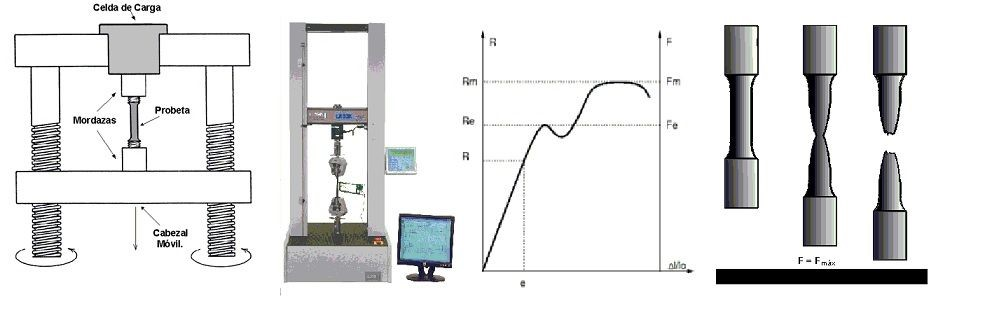
\includegraphics[width=9cm]{imagenes/primera.png}
		\caption{Modelo de tracción simple [2]}
		\label{1}
	\end{figure}
	
	La determinación de las propiedades de tracción para plásticos reforzados y no reforzados a través del ensayo de tracción se encuentra regulado por la norma ISO 527. El ensayo regulado por ISO 527-2 se realiza en una máquina de ensayo universal aplicando una fuerza de tracción a una muestra (probeta) y midiendo varias propiedades del material de la probeta bajo tensión. El ensayo se realiza a velocidades de tracción que van de 1 a 500 mm/min hasta que la muestra falla (cede o se rompe). [3] Adicionalmente, permite medir muchas propiedades de tracción diferentes. La mayoría de las pruebas ISO 527-2 se realizan en una máquina de prueba universal de mesa como la Instron 3369. 
	
		\begin{figure}[!h]
		\center
		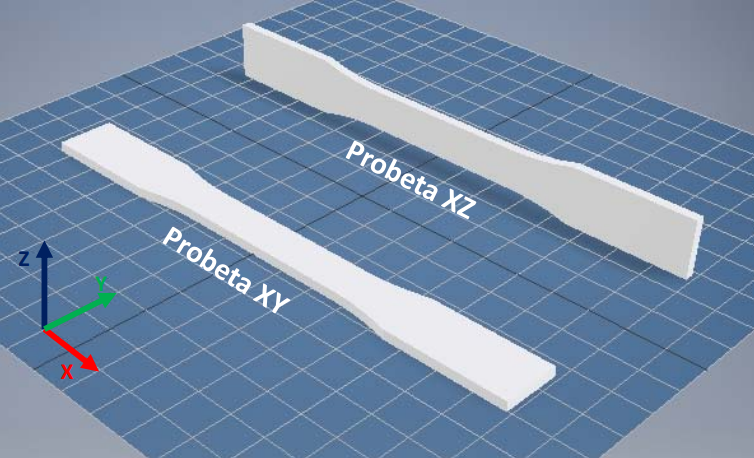
\includegraphics[width=7cm]{imagenes/segunda.png}
		\caption{Modelo de probetas [4]}
		\label{2}
	\end{figure}
		\begin{figure}[!h]
		\center
		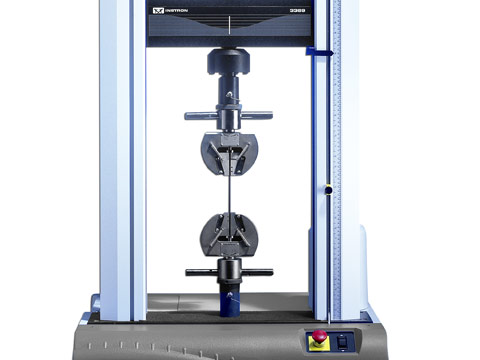
\includegraphics[width=5cm]{imagenes/tercera.png}
		\caption{Instron 3369 [5] }
		\label{3}
	\end{figure}
	
	
El Ácido Poliláctico (PLLA) es un polímero biodegradable muy usado en bioingeniería debido a sus propiedades mecánicas y biocompatibilidad. Este filamento también es muy implementado en otros campos de la industria debido a su versatilidad y ductilidad. El ácido poliláctico, es usado como filamento para la impresión 3D; es un polímero semicristiano de fácil manipulación, razón por la cual es uno de los más usados.

\section{Metodología}

Previamente, se imprimieron en 3D 5 probetas a densidades de 40\%, 60\%, 80\% y 100\% de filamento PLLA con dimensiones de 50 mm de largo, 10 mm de ancho y 4 mm de espesor y relleno de tipo panal.

\begin{figure}[!h]
		\center
		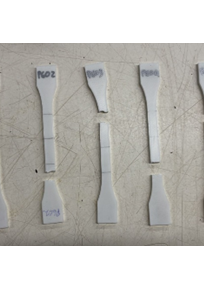
\includegraphics[width=7cm]{imagenes/muestras.png}
		\caption{Probetas de PLLA de 60\% de densidad   }
		\label{30}
	\end{figure}


Para la determinación de las propiedades tensiles (módulo de Young, esfuerzo de cedencia y esfuerzo máximo) de las probetas, cada grupo realizó el siguiente procedimiento: 

	\begin{enumerate}
	
    \item Se indica por software a la máquina de ensayos que se colocará una probeta. 
     \item     Se sujeta la probeta en la máquina de ensayos, de modo tal que el eje mayor de la probeta coincida con la dirección de extensión a través de la línea central del ensamblaje de agarre. Además, la probeta debe sujetarse de manera que se evite el deslizamiento con respecto a las mordazas de agarre, y éstas deben sujetarla con suficiente fuerza para soportar la prueba sin causar fractura prematura en la probeta. 
      \item     Se colocan las puntas del extensómetro justo en los límites del área de la probeta donde se desea medir la deformación. 
       \item     Mediante software, se prepara a la máquina de ensayos para la prueba de deformación. El software registra los datos de esfuerzo y deformación en cada paso hasta que la probeta se rompe. 
    
    	\end{enumerate}
    	
    	\begin{figure}[!h]
		\center
		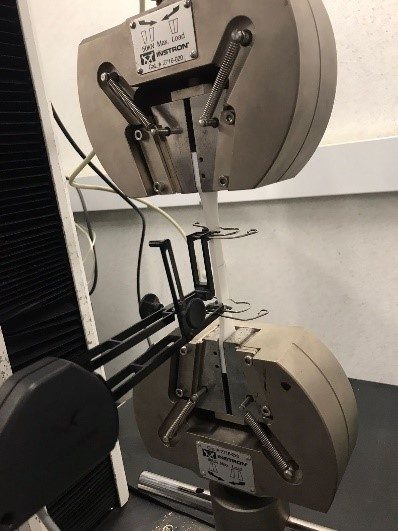
\includegraphics[width=5cm]{imagenes/ensayo1.png}
		\caption{ Montaje ensayo de tracción    }
		\label{31}
	\end{figure}
	
	\begin{figure}[!h]
		\center
		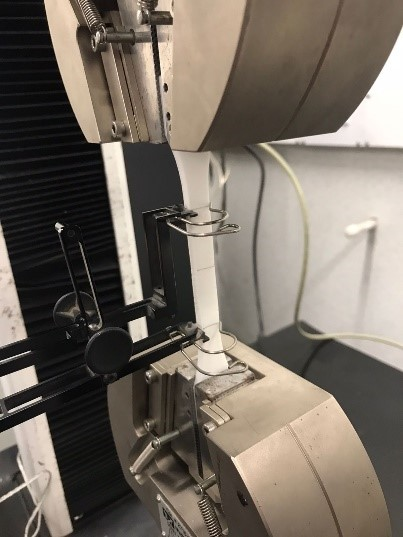
\includegraphics[width=5cm]{imagenes/ensayo2.png}
		\caption{ Montaje ensayo de tracción   }
		\label{32}
	\end{figure}
 
Para la obtención de las propiedades de tracción, se tomaron en cuenta las definiciones y procedimientos indicados en la ISO 527, parte 1. 

Para el módulo de Young, se obtuvo la pendiente de la curva de esfuerzo/deformación en el intervalo de la deformación e1 = 0.05\% y e2 = 0.25\%. 

Así mismo, para la obtención del esfuerzo de cedencia, se buscó el primer punto en el cual la pendiente de la curva de esfuerzo/deformación era negativa, es decir, el punto en el que el esfuerzo disminuye por primera vez. 

Para la obtención del esfuerzo último, se buscó el primer punto en el cual existe un decremento en el esfuerzo dentro de la región plástica de la curva. 

\section{Resultados}
	
Se recibieron 20 archivos CSV correspondientes a 4 grupos con 5 muestras de una densidad especifica de PLLA. Nuestro grupo era el grupo 1 con una densidad de 60\%, el grupo 2 tenía una densidad del 40\%, el grupo 3 del 100\% y el grupo 4 del 80\%. Los archivos se abrieron en excel, se cambió el punto decimal de coma a punto, se eliminaron las filas irrelevantes para el análisis de los datos y se volvieron a guardar los archivos CSV en el formato adecuado para procesarlos en R. 

Se cargaron los 20 archivos en R y se procedió a hacer una limpieza de los datos para eliminar aquellos valores con punto decimal faltante que no permitían ver las curvas de esfuerzo-deformación. Este código en R se encuentra anexo en un link al final de este documento. 

\subsection{Resultado probetas usadas por el grupo: }
En una sola figura se graficó el Esfuerzo de tracción con respecto a la Deformación de las 5 muestras de 60\% de densidad, además se graficaron líneas verticales mostrando la zona de comportamiento elástico del material entre 0.05\%-0.25\% de los datos, para identificar la región que se utilizó para hacer la regresión lineal más adelante. Se identificó el punto máximo de esfuerzo de esta grafica como el esfuerzo de cedencia del material y el punto antes de la ruptura como el punto de esfuerzo último del material. 

	\begin{figure}[!h]
		\center
		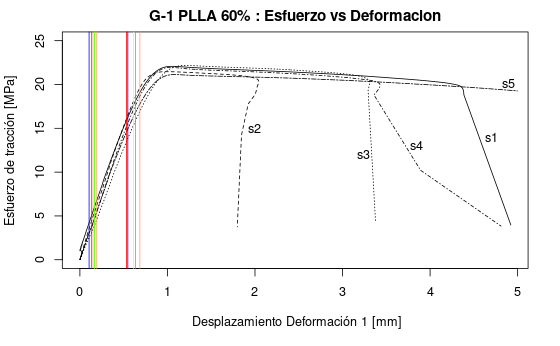
\includegraphics[width=9cm]{imagenes/grafica.png}
		\caption{Gráficas curvas de esfuerzo-deformación de las probetas usadas por el grupo.}
		\label{4}
	\end{figure}
	
	\subsection{Módulo de Young para los 4 grupos:  }
Se realizó la regresión lineal de todos los experimentos de cada grupo y el coeficiente que representa la pendiente de la recta de cada muestra se obtuvo. Para cada grupo se calculó el módulo de Young promedio y su desviación estándar. 

	\begin{figure}[!h]
		\center
		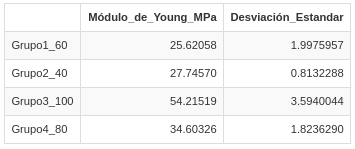
\includegraphics[width=8cm]{imagenes/young.png}
		\caption{Módulo de elasticidad (en todos los casos promedio y desviación estándar) }
		\label{5}
	\end{figure}
	
	\subsection{Esfuerzo último para los 4 grupos:  }
Para determinar el esfuerzo último eliminamos en promedio los ultimos 5 valores del conjunto de datos que presentaban una caída súbita en el esfuerzo, con el fin de obtener una gráfica con el último punto ubicado en el momento que ocurrió la fractura de la muestra. 

Luego se determinó el esfuerzo ultimo como el último esfuerzo soportado por la pieza. Para cada grupo se calculó su media y su desviación estándar. 

	\begin{figure}[!h]
		\center
		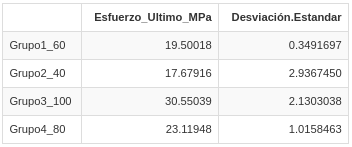
\includegraphics[width=8cm]{imagenes/ultimo.png}
		\caption{Esfuerzo ultimo (en todos los casos promedio y desviación estándar) }
		\label{6}
	\end{figure}
	
	
\subsection{Esfuerzo de cedencia para los 4 grupos: }
Este esfuerzo se halló simplemente detectando el esfuerzo máximo en cada muestra, para cada grupo se promedió y se halló la desviación estándar.  

	\begin{figure}[!h]
		\center
		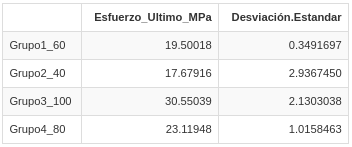
\includegraphics[width=8cm]{imagenes/ultimo.png}
		\caption{Esfuerzo de cedencia (en todos los casos promedio y desviación estándar) }
		\label{1}
	\end{figure}
		
		

\section{ANALISIS Y DISCUSION}

En la práctica, el parámetro variable de estudio fue la densidad de relleno en la probeta, esta representa la cantidad de material que se deposita en los contornos, su función es evitar movimientos relativos entre los mismos y otorga robustez a las piezas. 

Las propiedades mecánicas de las muestras de PLA con respecto a la densidad dependen de tres aspectos principales: las propiedades mecánicas de los filamentos; la fuerza de unión entre capas y las fuerzas de unión entre los filamentos de la misma capa. La disminución del relleno deriva en la perdida de fuerza de unión entre los filamentos de una misma capa, independientemente de la distancia entre los filamentos de esta, que es el efecto directo de la reducción de la densidad del relleno. Esto explica en cierto modo porque el efecto de cambio de densidad es más notorio cuando se reduce del 100\% a cualquier otro valor, esto se puede observar de la tabla 1 a la 3, donde el cambio del grupo3 es mucho más abrupto con respecto a los cambios que hay entre las otras densidades (80 a 60, 6 0 a 40 y 40 a 20). Un segundo hecho explicativo que podría explicar el cambio podría estar relacionado con el tamaño de las probetas, lo que significa que su comportamiento mecánico está “Influenciado” por su piel y, en menor medida, el relleno, que sólo está compuesto por unas pocas capas. 

Una observación muy importante a realizar es que la norma no hace mención del “esfuerzo último”, sino del “esfuerzo de ruptura”. Dado que las instrucciones para la realización de este reporte solicitan la obtención del esfuerzo último, se obtuvieron los datos del esfuerzo de ruptura y se reportaron como esfuerzo último. 
	
   \section{CONCLUSIONES}
 
 	\begin{enumerate}
 
  \item El porcentaje de material de PLLA en la probeta afecta los valores de módulo de elasticidad, el esfuerzo de cedencia y el esfuerzo ultimo.  
   \item Los resultados, se pudieron ver afectados por la variabilidad de los datos experimentales, la cual depende de factores como la calidad de impresión, el método implementado para el cálculo del área transversal, los posibles errores instrumentales en los equipos de medición, la máquina de ensayos y en la calibración de las impresoras 3D que fueron empleadas para la fabricación de las probetas. 
    \item Los módulos de Young calculados con la regresión lineal fueron consistentes a lo largo de las muestras y esto se refleja en la desviación estándar que es muy pequeña. Al igual que los esfuerzos de cedencia y últimos, se obtuvieron valores muy similares entre los grupos. 
    
    	\end{enumerate}

\section{ANEXOS}

\subsection{Codigo de R}
    Link códigos y graficas de los datos en R: https://rpubs.com/willandru/962976 

\ifCLASSOPTIONcaptionsoff
  \newpage
\fi


\begin{thebibliography}{1}


 \bibitem{IEEEhowto:Monteria}
  N. Özkaya, D. Leger, D. Goldsheyder y M. Nordin, Fundamentals of Biomechanics Equilibrium, Motion, and Deformation, Switzerland: Springer, 2018. 
 

 \bibitem{IEEEhowto:Monteria}
areatecnologia., area tecnologia, [En línea]. Available: https://www.areatecnologia.com/materiales/ensayo-de-traccion.html. [Último acceso: 02 11 2022].
 \bibitem{IEEEhowto:Monteria}
E. Lawrence, INSTRON, [En línea]. Available: https://www.instron.com/en/testing-solutions/iso-standards/iso-527-2. [Último acceso: 02 11 2022].
 \bibitem{IEEEhowto:Monteria}
M. J. C. Loaiza, P. G. Díaz y e. al, Influencia de la posición de impresión y la densidad de relleno, Revista Ingenierias Universidad de Medellín, vol. 2, p. 15, 2020. 
 \bibitem{IEEEhowto:Monteria}
UMBC, UMBC, MicroMaterials Characterization Lab, [En línea]. Available: https://mmc-lab.umbc.edu/resources/instron/. [Último acceso: 02 11 2022].

 \bibitem{IEEEhowto:Monteria}
Travieso-Rodriguez JA, Jerez-Mesa R, Llumà J, Traver-Ramos O, Gomez-Gras G, Roa Rovira JJ. Mechanical Properties of 3D-Printing Polylactic Acid Parts subjected to Bending Stress and Fatigue Testing. Materials (Basel). 2019 Nov 22;12(23):3859. doi: 10.3390/ma12233859. PMID: 31766653; PMCID: PMC6926899.


\end{thebibliography}



\end{document}
